\documentclass{beamer}
 
\usepackage[utf8]{inputenc}
\usepackage{xeCJK}
\setCJKmainfont{IPAMincho}
\graphicspath{ {images/} }
 
 
\title{Learning Transliteration without Parallel Data}
\author{Derick Anderson and Timothy Gillis}
\date{Spring 2019}
 
 
 
\begin{document}
 
\frame{\titlepage}
 
\begin{frame}
  \frametitle{Project Idea}

  \begin{itemize}
  \item Transliterate from English to Japanese without parallel data
  \item Do that using recent work on word translation without parallel data
  \end{itemize}

\end{frame}

\begin{frame}
  \frametitle{Background - Transliteration}

  \begin{itemize}
  \item To represent a word in a script different from that it was originally
    written in
  \item For some script pairs it's as easy as a table lookup
    \begin{itemize}
      \item E.x. Middle English alphabet ``þe'' -> Modern English alphabet ``the''
    \end{itemize}

  \item For some script pairs it requires some thinking
    \begin{itemize}
    \item In Japanese, primarily approximate pronunciation but also consider
      spelling
    \item Key for our project: transliterated words are written in a specific
      script called katakana (in modern times anyway)
    \item E.x: Edinburgh -> エディンバラ, Boston -> ボストン
    \end{itemize}

  \item Usually learning transliteration requires at least parallel data,
    i.e. text which means the same thing in both scripts of interest
  \end{itemize}

\end{frame}

\begin{frame}
  \frametitle{Background - Word Translation w/o Parallel Data}
  Conneau et al propose the following for unsupervised word translation:
  \begin{itemize}
    \item A domain-adversarial approach to minimize $\|WX-Y\|_2$ where $W$ is
      a linear mapping and $X,Y$ are monolingual word embeddings.
    \item A refinement procedure where a synthetic vocabulary is constructed
      with the learned $W$ to apply the Procrustes solution (i.e.
      min $\|WX-Y\|_2 = UV^T$, where $U\Sigma V^T = SVD(YX^T)$).
      \begin{itemize}
        \item This can be used with ground truth data as a supervised
          approach as well.
      \end{itemize}
    \item A similarity measure for word translation which mitigates hubs in
      nearest-neighbor graphs. In this case, target words that are translations
      for many source words.
    \item An unsupervised validation criterion for model selection: mean
      cosine similarity between translations of most frequent 10,000 words.
  \end{itemize}

\end{frame}

\begin{frame}
  \frametitle{Method}
  \begin{itemize}
  \item Learn word translations from Japanese to English
  \item Find the English translations of Japanese katakana words by translating
    the most frequent words in the Japanese embedding vocabulary.
  \item Train the transliteration model on those pairs
    \begin{itemize}
    \item Our transliteration model is straightforward: an RNN encoder-decoder with
      attention
    \end{itemize}
  \item Evaluate on katakana pairs from a dictionary Facebook Research provides
  \end{itemize}
\end{frame}

\begin{frame}
  \frametitle{Results}
  \begin{itemize}
  \item Japanese-English word translation does not work: Purely unsupervised
    approach gets 0 precision at k=1, supervised approach gets 7.72 precision
    at k=1.
    \begin{itemize}
    \item The domain-adversarial approach is highly sensitive to hyper-parameters.
    \item The model selection metric correlates less with word translation
      accuracy as languages get further apart.
    \item The Japanese word embedding tokens seem to be noisy to begin with.
    \end{itemize}
  \item While Conneau et al's approach aims to mitigate hubs, we do not have
    sufficient resources to hold the entire vocabulary in memory, causing many
    words to be incorrectly translated as adverbs, prepositions, etc.
  \item Learning on translation pairs we generate get's us to 0.5\% accuracy,
    adding in transfer learning pushes that to 1.2\%.
  \end{itemize}
\end{frame}

\begin{frame}
  \frametitle{Fallback Exploration - Timothy}
  How well does the unsupervised metric correlate with word translation accuracy?
  \begin{itemize}
  \item Conneau et al. claim it correlates well, however they only show one example
    as proof without specifying the language pair.
  \end{itemize}
  \begin{columns}
    \column{0.5\textwidth}
    \begin{table}
      \begin{tabular}{l | c | c }
      Language & $\text{R}^2$ & P@1 \\
      \hline \hline
      Spanish & 0.8581 & 83.3 \\
      Korean & 0.7754 & 13.2 \\
      French & 0.7722 & 82.1 \\
      Chinese & 0.0237 & 31.4 \\
      Japanese & -0.2715 & 0.0
      \end{tabular}
    \end{table}
    \column{0.5\textwidth}
      \frame{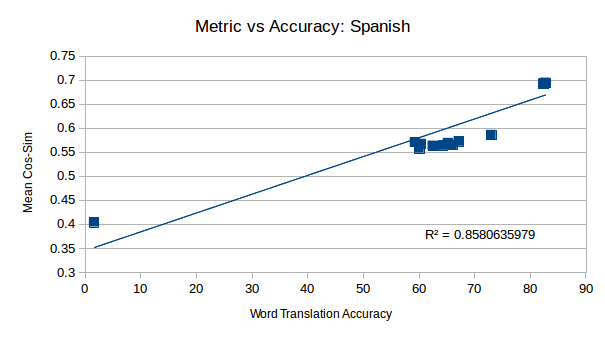
\includegraphics[width=\textwidth]{spanishCorr}} \\
      \frame{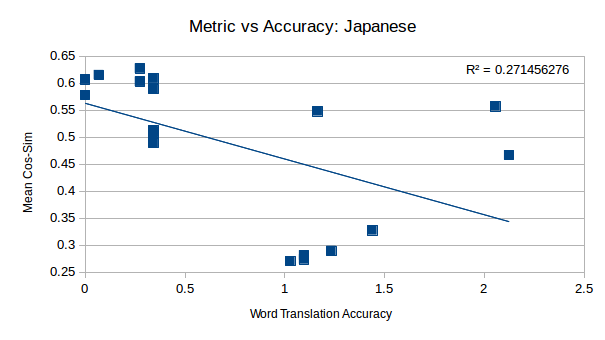
\includegraphics[width=\textwidth]{japaneseCorr}}
  \end{columns}
\end{frame}

\begin{frame}
  \frametitle{Fallback Exploration - Derick}
  \begin{itemize}
  \item English -> Japanese transliteration is affected by both the spelling and
    pronunciation of the English word
  \item The neural transliteration paper
    \footnote{https://arxiv.org/abs/1610.09565} we use as a baseline only
    incorporates the written form of a word
  \item Can we improve transliteration accuracy with a multi-task learning
    setup of also predicting the pronunciation of a word?
  \item Yes, we can: informal results suggest an about 6\% accuracy jump (from
    the mid-forties).
  \item Formal results on the accuracy benefit and an analysis of the best way
    to do the multi-task learning are in process
  \end{itemize}
\end{frame}

\begin{frame}
  \frametitle{Conclusions}
  \begin{itemize}
  \item Conneau et al.'s unsupervised word translation approach completely fails
    with the Japanese-English language pair.
  \item Their proposed similarity metric only correlates well with accuracy when
    the source/target languages are similar.
  \item The translation data generated from the word translation model are too
    noisy for our model to learn transliteration
  \item Multi-task learning to also predict the pronunciation of an English word
    improves the accuracy of English -> Japanese transliteration
  \end{itemize}
\end{frame}

\end{document}
%%% Local Variables:
%%% mode: latex
%%% TeX-engine: xetex
%%% TeX-master: t
%%% End:
